\documentclass[
	DIV=9,						% Einstellung für den Seitenaufbau (Standardwert)
	bibliography=totoc, 		% Literaturverzeichnis ins Inhaltsverzeichnis
	listof=totoc,				% Abbildungs- und Tabellenverzeichnis ins Inhaltsverzeichnis
	abstract=true,				% Mit Abstract
	11pt,						% Schriftgröße
]{scrartcl} 					% scrartcl für kurze Arbeiten (Achtung: es steht kein \chapter zur Verfügung)
%]{scrreprt} 
%saubere Zeilenumbrüche in URLs
\usepackage[hyphens]{url}
\sloppy

% Euro-Symbol
\usepackage{eurosym}
\usepackage{smartdiagram} %für Smart-Art zur SHA

\usepackage[utf8]{inputenc}		% Eingabedaten liegen im UTF8-Format vor
\usepackage[T1]{fontenc} 		% Ausgabezeichensatz
\usepackage{lmodern}			% Zeichensätze für die Arbeit
% -------------------------------------------------------------------------------
\usepackage[fleqn,				% Mathematische Formeln linksbündig eingerückt
			%leqno,				% Gleichungsnummerierung links
			intlimits,			% Integralgrenzen oben und unten
			]{amsmath}			% Mathematik
% -------------------------------------------------------------------------------
\usepackage[ngerman, english]	% Auswahl der Sprachen, für die Layout- und Umbruchregeln bekannt sein sollen
					{babel}		% Die Sprachen werden mit \selectlanguage{} ausgewählt. Die aktuell Wahl ist ngerman


\usepackage{graphicx}			% Einbinden von Grafiken
								% da die Kompilierung über 'pdflatex' erfolgt, stehen '.jpg', '.png' und '.pdf'
								% als Grafikformate zur Verfügung
%\usepackage{textcomp}  %für DollarZeichen
% Für Beispiel
\usepackage{blindtext}


% Paket aus den KOMA-Klassen für die Einstellungen der Kopf- und Fußzeilen
% Nachfolger von scrpage2
% Eine Alternative wäre das Paket 'fancyhdr'
% Siehe dazu Kapitel 5 im SCRGUIDE
\usepackage{scrlayer-scrpage}
\automark{section}			% \automark -> Kapitel 5.5 im SCRGUIDE
\clearscrheadfoot			% Kopf- und Fußzeilen leeren
\ohead[]{\headmark}			% \ohead -> Abbildung 5.1 im SCRGUIDE
                            % \headmark -> Kapitel 5.5 im SCRGUIDE
% \ihead{\includegraphics[height=\baselineskip]{img/hpi_logo.png}}
                            % \ihead -> Abbildung 5.1 im SCRGUIDE
\ofoot[\pagemark]{\pagemark}			% \ofoot -> Abbildung 5.2 im SCRGUIDE
                            % \pagemark -> Kapitel 5.5 im SCRGUIDE
\setkomafont{pagehead}{\scshape} % Siehe Beispiel auf Seite 237 im SCRGUIDE
\addtokomafont{pagehead}{\bfseries} % Befehle \setkomafont und \addtokomafont -> Kapitel 3.6 im SCRGUIDE
%\addtokomafont{pagehead}{\color{green}} % Befehle \setkomafont und
% \addtokomafont -> Kapitel 3.6 im SCRGUIDE \addtokomafont{section}{\color{red}} % Befehle \setkomafont und \addtokomafont
% -> Kapitel 3.6 im SCRGUIDE
\pagestyle{scrheadings}
\setlength{\headheight}{24pt}
\setlength{\footheight}{24pt}


% Wasserzeichen auf dem Dokument -----------------------------------------------------------------
%	Das ist dafür gedacht, dass man Vorabexemplare herausgeben kann, ohne dass sie später
%	als Originale herumgereicht werden.
% \usepackage{draftwatermark}							% Wasserzeichen immer in grau
% \SetWatermarkLightness{.95}							% Grauwert, zwischen 1 (weiß) und 0 (Schwarz)
% \SetWatermarkAngle{60}								% Winkel, um den das Wasserzeichen gedreht worden ist.
% \SetWatermarkFontSize{5cm}							% Schriftgröße beim Wasserzeichen (max 5cm)
% \SetWatermarkScale{.5}								% nachträgliche Skalierung
% \SetWatermarkText{\sffamily\textbf{Stand: \today}}	% Wasserzeichentext

\usepackage[margin=1in]{geometry} 
% \usepackage[left=3cm,right=2.5cm,top=2.5cm,bottom=2.5cm]{geometry} 
\usepackage{xcolor}
\usepackage[]{todonotes}

% Korrekte Einheitendarstellung -------------------------------------------------------------
\usepackage[output-decimal-marker={,}, 	% Dezimal-Trennzeichen ist in Deutschland das Komma
			]{siunitx}


\usepackage{array} % einfache Erweiterungen für die Tabellenformatierungen
% ---------------------------------------------------------------------------------
% Wenn man unbedingt den Zeilenabstand erhöhen muss, dann über das Paket setspace
\usepackage{setspace}
\onehalfspacing

\usepackage{paralist}%für Aufzählungsumgebungen

%Abbildungen
\usepackage{caption}
\usepackage{subcaption}

% Abkürzungverzeichnis
\usepackage[printonlyused	% nur die Abkürzungen aufführen, die auch verwendet werden
			]{acronym}


\usepackage[citestyle=authoryear,backend=biber,style=authoryear]{biblatex}
\bibliography{lit.bib}

% Nützliche Pakete
\usepackage{csquotes}		% Anführungsstriche
%\usepackage{relsize}		% Wenn man Zwischengrößen in den Schriftgrößen benötigt, bitte die Doku aufmerksam lesen
%\usepackage{listings}		% Für die Behandlung von Quellcode
%\usepackage{media9}		% Einbinden von Videos
%\usepackage{animations}	% Eigene Animationen
%\usepackage{attachfile2}	% Einbau von Dateien in die pdf-Datei
%\usepackage{xcolor}		% Damit man mit Farben umgehen kann, wird aber von vielen Paketen mit geladen (z.B. hyperref)
\usepackage{makeidx}\makeindex % Für ein Stichwortverzeichnis (es gibt auch eine Alternative namens xindy - glaube ich)
%\usepackage{titlesec}
%\makeatletter
%\renewcommand\paragraph{\@startsection{paragraph}{4}{\z@}%
%	{-2.5ex\@plus -1ex \@minus -.25ex}%
%	{1.25ex \@plus .25ex}%
%	{\normalfont\normalsize\bfseries}}
%\makeatother
\setcounter{secnumdepth}{3} % how many sectioning levels to assign numbers to
\setcounter{tocdepth}{3}    % how many sectioning levels to show in ToC
% für paragraph als subsubsubsection
% Für sehr interessierte und engagierte Leute ;)
\usepackage{tikz}			% Grafiken mit LaTeX - extrem mächtig und schön (Alternative wäre psstricks)
\usetikzlibrary{arrows,shapes,positioning,shadows,trees}
\usetikzlibrary{shadings}
\usepackage{smartdiagram} %smart art diagramme
\usepackage{adjustbox}
\usepackage[final]{pdfpages} %für includepdf
%\usetikzlibrary{shapes,snakes}
%\tikzstyle{every node}=[draw=black,thin,anchor=west, minimum height=2.5em]
% \usepackage{pgfplots}		% setzt auf TikZ auf (lädt es also) und ist speziel für die Datenvisualisierung
% \usepackage{ifthen}		% (La)TeX bietet schon selber if-then-Möglichkeiten, durch das Paket werden sie angenehmer im Handling
% \usepackage{forloop}		% auch Schleifen sind möglich

% Laut Dokumentation sollte diese Paket als Letztes eingebunden werden.
\usepackage[hidelinks,						% Links im pdf-Dokument nicht farblich hervorheben (gilt nur für die Darstellung auf dem Bildschirm)
			pdfauthor={Tobias Wuttke}, % Schreibt den Autor in die PDF-Datei
			]{hyperref}

\newcounter{speichereRoemischeZahl}
\def\mytitle{The effects of prototyping and Lego Serious Play \\ in leadership seminars} 

\usepackage{graphicx}
\usepackage{lscape}

% %Komma zwischen Fußnoten, gibt leider eine Warnung
% \usepackage[multiple]{footmisc}

%Seiten im Querformat (große Tabellen die es vermutlich gibt)
%\usepackage{pdflscape}
 
%Tabellen skalieren
%\usepackage{tabularx}
%\usepackage{tabu} %rowfont 
%\usepackage{longtable} %endhead
 
\newlength{\drop}

\usepackage{setspace}
\doublespacing

\begin{document}
    %\listoftodos
	\pagestyle{plain}
	\begin{titlepage}
    \drop=0.1\textheight
    \centering
    \vspace*{\baselineskip}
    \rule{\textwidth}{1.6pt}\vspace*{-\baselineskip}\vspace*{2pt}
    \rule{\textwidth}{0.4pt}\\%[\baselineskip] ausgeklammert am 29.09.2016
    {\Huge WAYFINDER\\
    \vspace*{12pt} %Geandert von 29.09.2016
    \LARGE \mytitle}\\[0.2\baselineskip]
    \rule{\textwidth}{0.4pt}\vspace*{-\baselineskip}\vspace{3.2pt}
    \rule{\textwidth}{1.6pt}\\[\baselineskip]
    \scshape
    Berlin, \today\par
    \vspace*{2\baselineskip}
    Created by: \\[\baselineskip]
    {\Large Lukas Hüller (796454)\par}\bigbreak Supervisors:\bigbreak 
    {\Large Klaudia Thal \\ Dr. Claudia Nicolai \\ Dr. Martin Schwemmle\par}\bigbreak\bigbreak
    \vfill
    
\includegraphics[width=0.5\textwidth]{img/hpi_dschool_logo.jpg}
  \end{titlepage}
    \pagenumbering{gobble}% Remove page numbers (and reset to 1)
\clearpage
\begin{abstract}
\blindtext
\end{abstract}
	\pagestyle{scrheadings} 
	\pagenumbering{Roman}
	\tableofcontents
	\newpage
	\setcounter{speichereRoemischeZahl}{\value{page}}
	\pagenumbering{arabic}
	\section{Motivation}
Introduction into the topic and its relevance, including the personal relevance for you: Your personal insight that triggered the selection of this topic – why is it meaningful to you? \\
\vspace{2cm} \\
\blindtext\newpage
	\section{Prototyping \& LSP: Status Quo}\label{sec:statusQuo}

\subsection{What Is Prototyping \& LSP?}
What it is. What are its roots, basic components, and consequences? \\
How is it embedded in its field? Why is it working? ... 
\begin{enumerate}
    \item Was charakterisiert Prototyping?
    \item Welche anderen Arten von Prototyping gibt es?
    \item Vorstellung Methode LSP \& Why is it working?
\end{enumerate}


\subsection{Where Is LSP Applied?}\label{ssec:application}
Where it’s applied. How / Where is it currently applied?\newpage
	\section{Implementierung von LSP im Wayfinder Seminar}

\subsection{konkrete Anwendung von LSP}
\label{implementation}

Im Wayfinder wurde die LSP Methode zum Prototypisieren unserer Zukunftspläne genutzt. 

In der ersten Woche des Seminars analysierten wir unsere langfristigen Lebensziele. Dazu untersuchten wir das eigene Weltbild und formulierten es aus. Dies half dabei, unsere Lebensziele für in 20-30 Jahren zu definieren. Zudem lernten wir in der ersten Woche unsere Triade (ein festes Dreierteam für den Rest des Workshops) kennen. Da bis zu diesem Tag nicht alle Teilnehmenden das LSP Set erhalten hatten, konnte die Methode in der ersten Woche noch nicht eingesetzt werden. 

In der zweiten Woche betrachteten wir dann unsere Ziele für die kommenden 5 Jahre etwas genauer. Dabei gingen wir erstmals von unserer aktuellen Situation aus und überlegten, wo es Überschneidungen mit den Lebenszielen gibt. Diese fassten wir auf dem so genannten ``Coherence-Board‘‘ zusammen. Zum Prototypisieren der Lebensziele wurde dann die LSP-Methode wie folgt angewendet. Anfangs stiegen wir mit kurzen Übungen ein, um uns mit den Steinen und der Methode vertraut zu machen. Im Anschluss daran bauten wir das Modell ``My 2020‘‘. Dieses Modell sollte ausdrücken, welche Ziele oder Wünsche noch in diesem Jahr in Erfüllung gehen sollen. In meinem Fall beschrieb es vor allem den Einklang von Studium, Beruf und Zeit für Urlaub sowie Privatleben. Ein Foto des entstandenen Prototyps ist im Anhang (Abbildung \ref{fig:week2}) beigefügt.

Das Motto der dritten Wayfinder-Einheit lautete ``Act now''. Alle Teilnehmenden entwickelte einen konkreten Plan, wie sie in den kommenden Monaten ihr Leben verbessern wollen. Auch diese entstandene Ideensammlung wurde am Ende wieder mittels LSP prototypisiert. Aufgrund des Feedbacks, dass mein erstes Modell (siehe Abbindung \ref{fig:week3}) zu eingeengt und starr wirkt, habe ich mich für ein modulareres Modell entschieden. Ich versuchte mit einzelnen Bausteinen einen Ort abzubilden, an dem ich sowohl das Arbeiten als auch die Entspannung und den Urlaub vereinen kann. Die Blumen im oberen Bereich des Modells symbolisieren, dass dieser Ort nicht die Großstadt ist, in der ich momentan lebe. Der Propeller soll darstellen, dass durchgehend die Möglichkeit besteht, wieder nach Hause zurückzukehren oder den Ort zu wechseln.


In der letzten Woche nutzten wir die LEGO-Bausteine zum Erstellen unseres finalen Wayfinder-Modells (siehe Abbildung \ref{fig:week4}). Hierbei versuchte ich alle Säulen, die meine Zukunftspläne beeinflussen, in einem Modell abzubilden. Daher entschied ich mich, einen 4-zackigen Stern zu bauen, welcher gleichzeitig als Wippe fungiert. Somit soll ausgedrückt werden, dass wenn sich die Person einem Thema widmet, die anderen Säulen sprichwörtlich ``In der Luft hängen‘‘. Die vier Säulen meines Zukunftsmodells setzen sich aus Urlaub, dem Leben in der Heimat mit Eltern und Freunden, dem Studium und dem beruflichen Alltag zusammen. Die Balance zwischen diesen Punkten wird durch meinen finalen Prototyp abgebildet. \newline

Besonders interessant war für mich, dass wir jede Woche unter völlig neuen Gesichtspunkten begannen, den Prototypen zu erbauen. Dennoch kam am Ende jedes Prototypings ein Modell heraus, welches dieselben vier Säulen wiederspiegelte. Die Art der Anordnung und die damit verbundenen Hintergrundgedanken änderten sich jedoch bei jeder Iteration. Aufgrund des Feedbacks, dass das erste Modell so einengend wirkt, wollte ich in der dritten Woche ein flexibles Modell, bei dem nicht alle Teile untereinander verbunden sind, konstruieren. Jedoch merkte ich, dass ich genau diesen Zusammenhang der Säulen benötige, um mich selbst von der Realisierbarkeit der Zukunftspläne zu überzeugen. Daher landete ich zuletzt mit dem Stern bei einem offenen Modell, bei dem alle Teile miteinander verbunden sind.

\subsection{andere Integrationsformen der Methode}

Wie im Abschnitt \ref{implementation} beschrieben, wurde die LSP-Methode mehrfach im Kurs angewendet. Auf der Suche nach anderen Implementierungsmöglichkeiten bin ich aufgrund der guten Anwendung (siehe dazu auch Abschnitt \ref{diskussion} auf Seite \pageref{diskussion}) im Seminar und dem ungewöhnlichen remote Setup lediglich auf Verbesserungsmöglichkeiten gestoßen.
Bei einer Vor-Ort-Variante des Workshops hätte es sich sicherlich angeboten, das Vorstellen der Prototypen in noch kleineren Gruppen vorzunehmen. Somit hätte man unter Umständen ein direkteres und umfangreicheres Feedback zum eigenen Prototyp erhalten.

Darüber hinaus würde ich die Methode LSP für ein morgendliches Warmup verwenden. Während der remote Workshops wurde täglich eine ``Zeit zum Einchecken‘‘ von 30 Minuten gewährt. Für diese Zeit wären eine oder zwei kleine Aufgaben mit den Lego-Sets denkbar, mit der die Teilnehmenden das richtige Mindset erlangen, um in den Tag zu starten. Hierbei würden sich Modelle zur aktuellen Gefühlslage oder der Zufriedenheit mit der Hausaufgabe gut zum Bauen eignen. Genau diese Themen wurden zu Beginn eines jeden Workshops mit allen Teilnehmenden besprochen.\newpage
	\section{Discussion}
\blindtext
	\newpage
	\singlespacing
	\pagenumbering{Roman}
	\setcounter{page}{\value{speichereRoemischeZahl}}
	\printbibliography[title={References}]
	\doublespacing
	\appendix % Anhang

    % Kapiteln mit Buchstaben beziffern
    %\renewcommand*\thechapter{\Alph{chapter}}
    \renewcommand{\thetable}{\Alph{table}}
    \setcounter{table}{0}
    \renewcommand{\thefigure}{\Alph{figure}}
    \setcounter{figure}{0}

\section{Anhang}

\begin{figure}[h]
    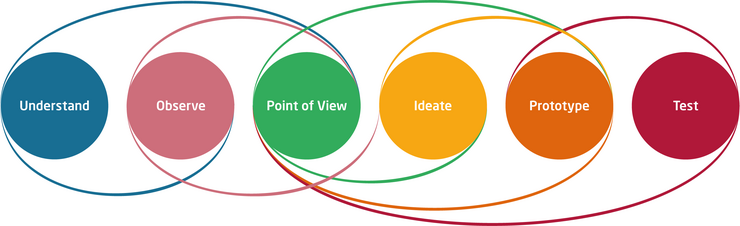
\includegraphics[width=\textwidth]{img/DT_process.png}
    \caption{The Design Thinking Process (\textcopyright ~HPI Academy)}
    \label{fig:dt_process}
\end{figure} 

\begin{figure}[h]
    \begin{center}
        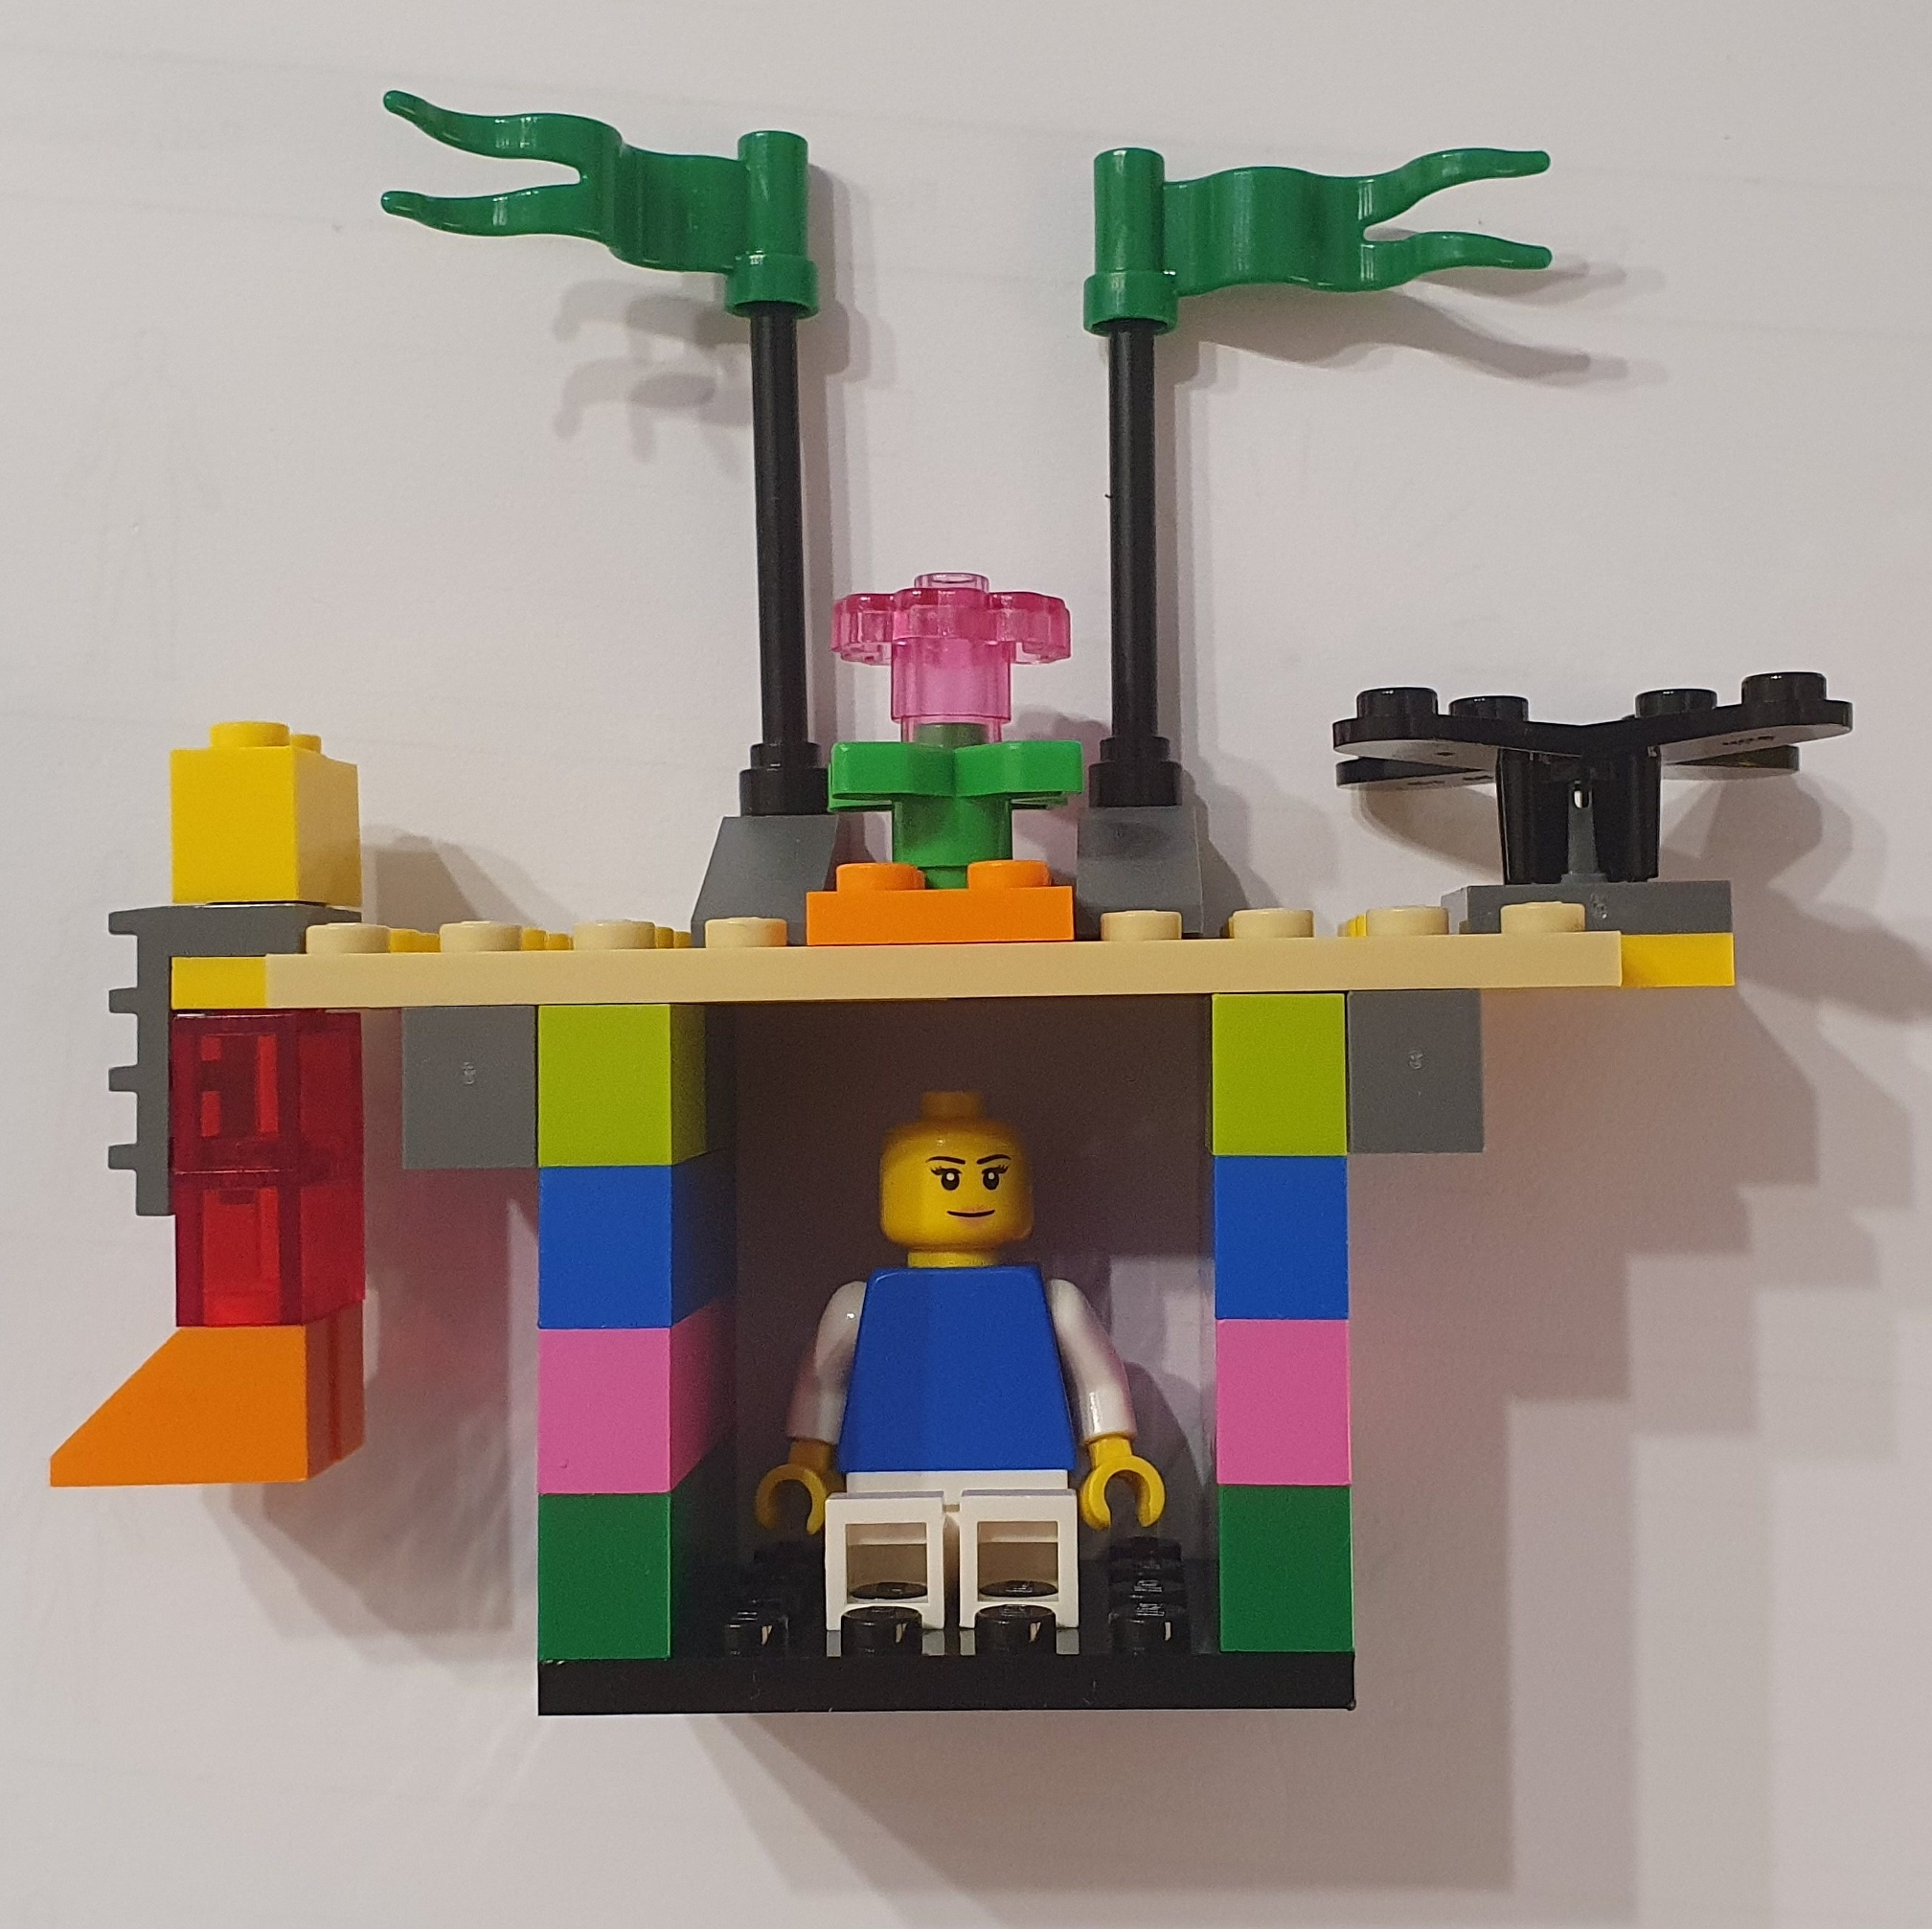
\includegraphics[width=7.5cm]{img/week_2.jpg}
    \end{center}
    \caption{``My 2020'' - Prototype of week 2}
    \label{fig:week2}
\end{figure} 
\begin{center}
    \begin{figure}[h]
        \begin{center}
            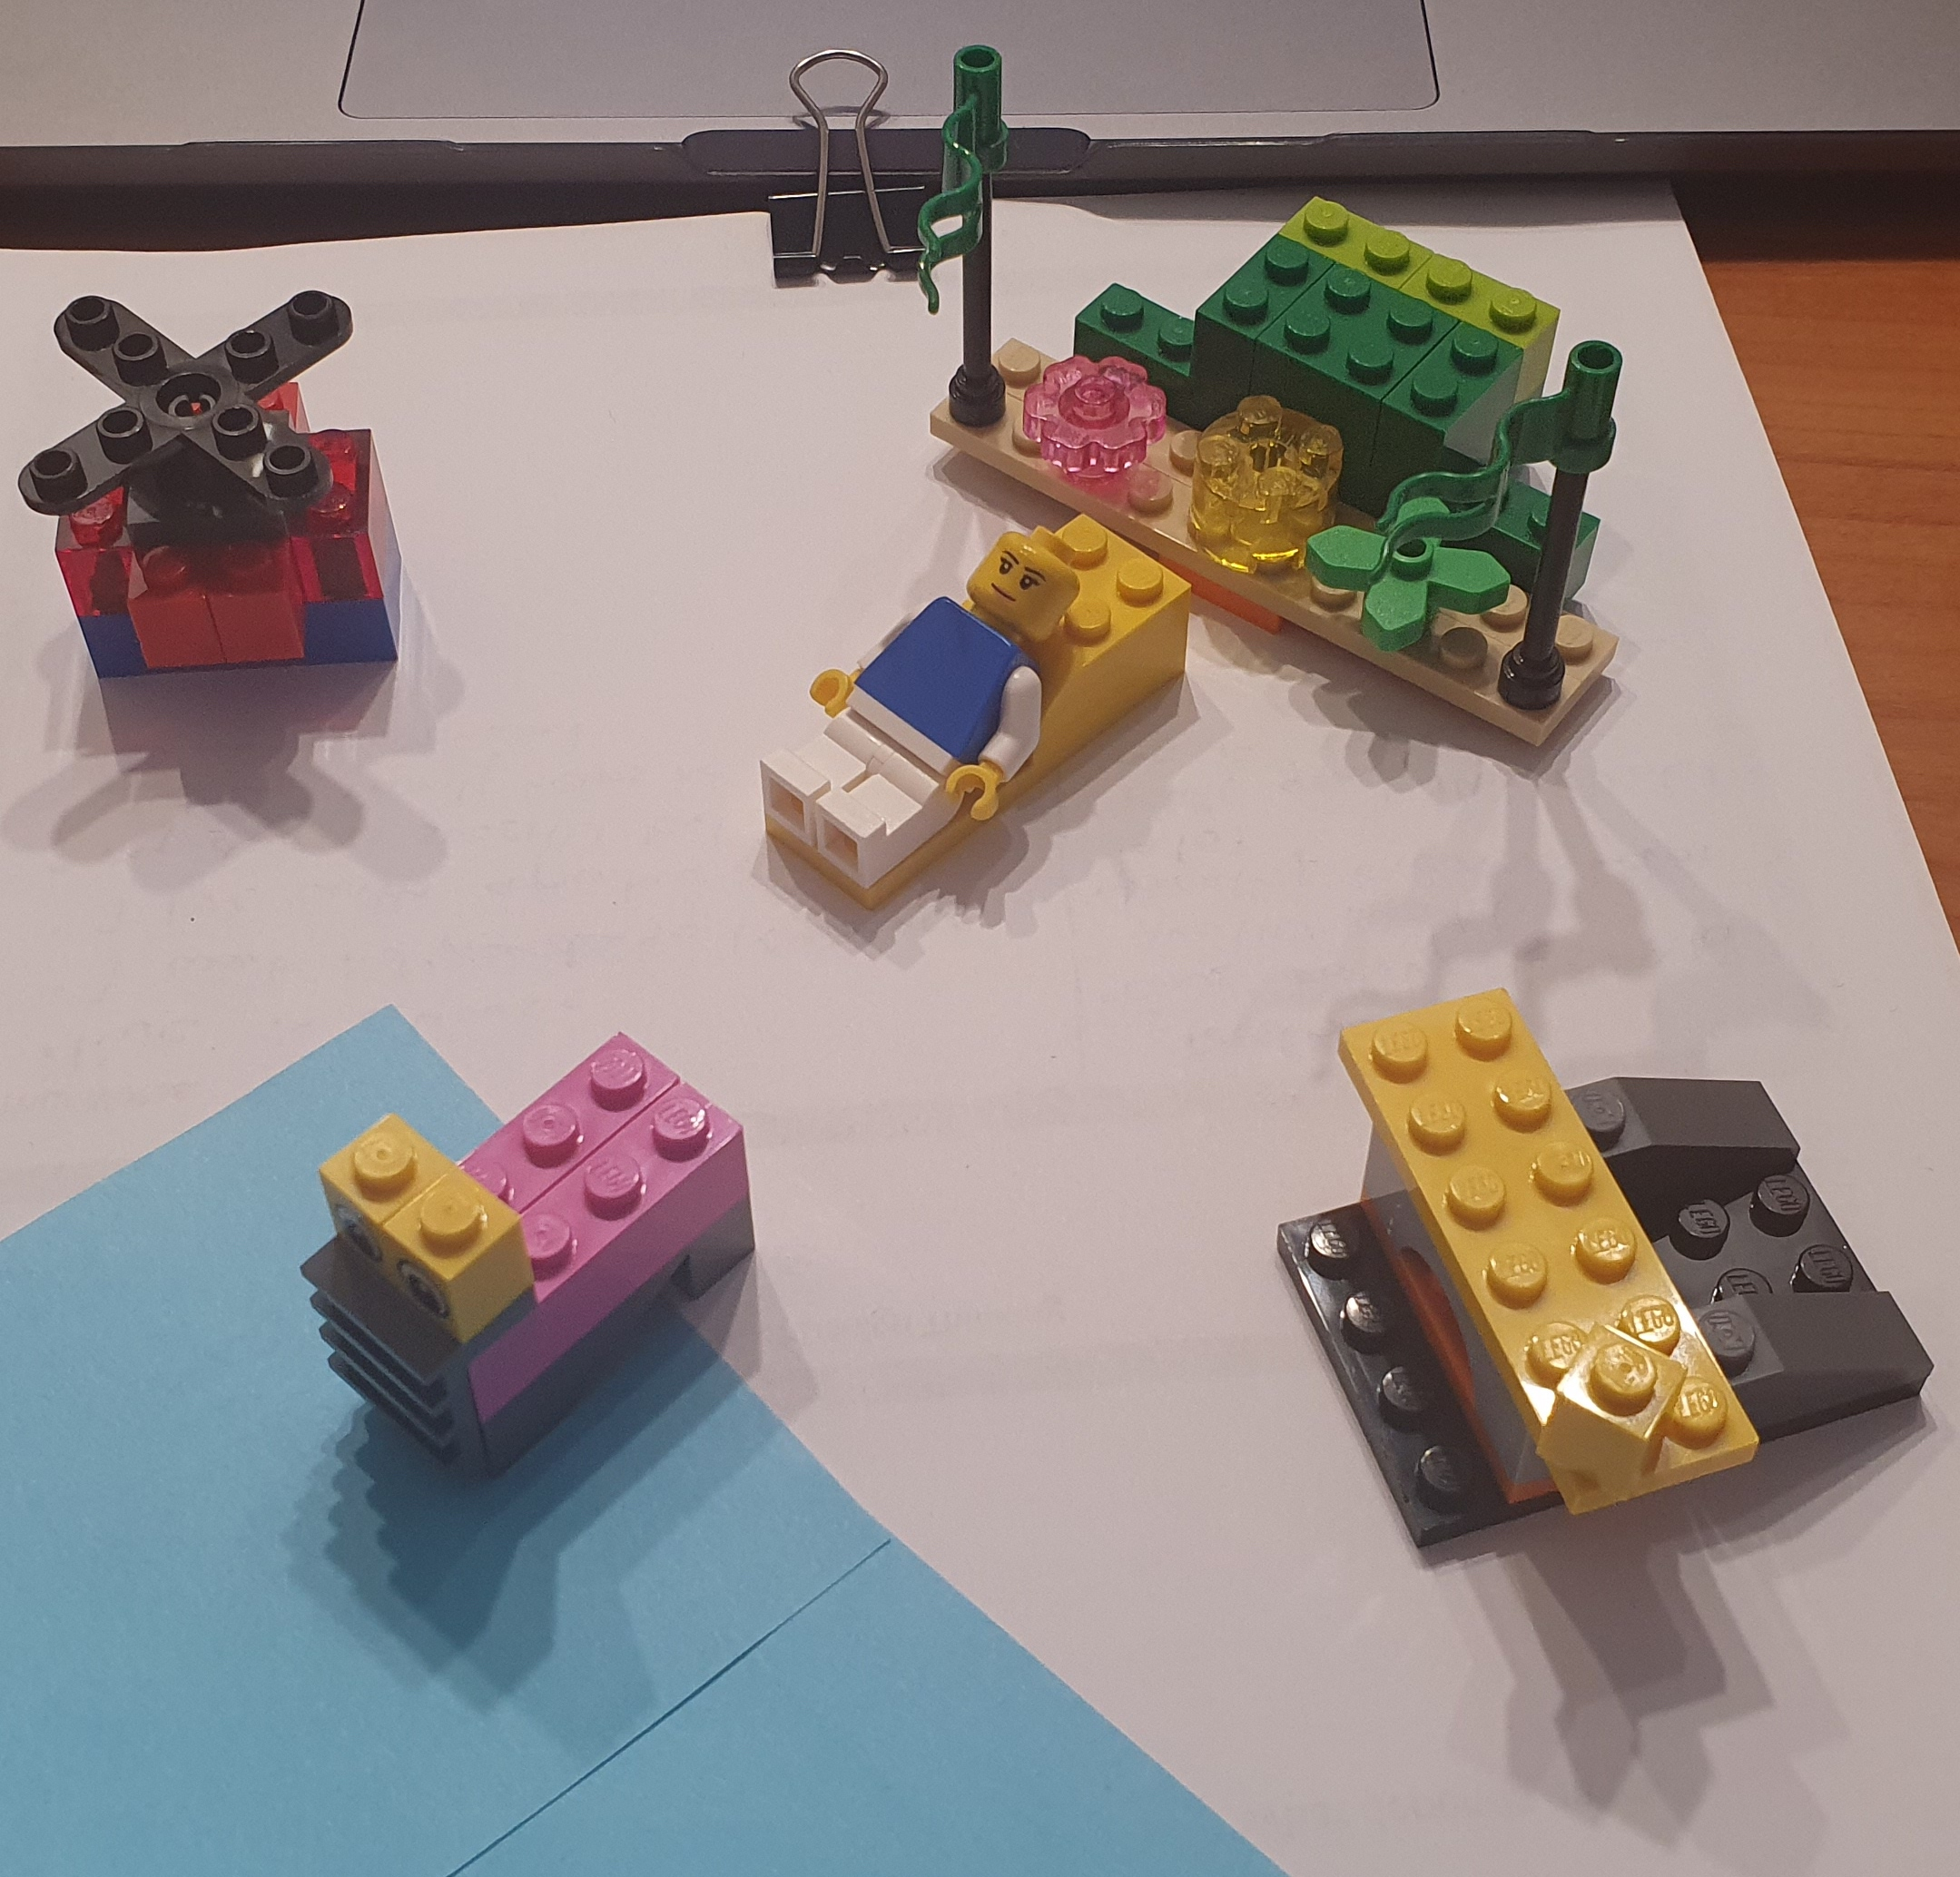
\includegraphics[width=7.7cm]{img/week_3_1.jpg}
        \end{center}
        \caption{``Working remote'' - Prototype of week 3}
        \label{fig:week3}
    \end{figure} 
    \vspace{2 cm}
    \begin{figure}[h]
        \begin{center}
            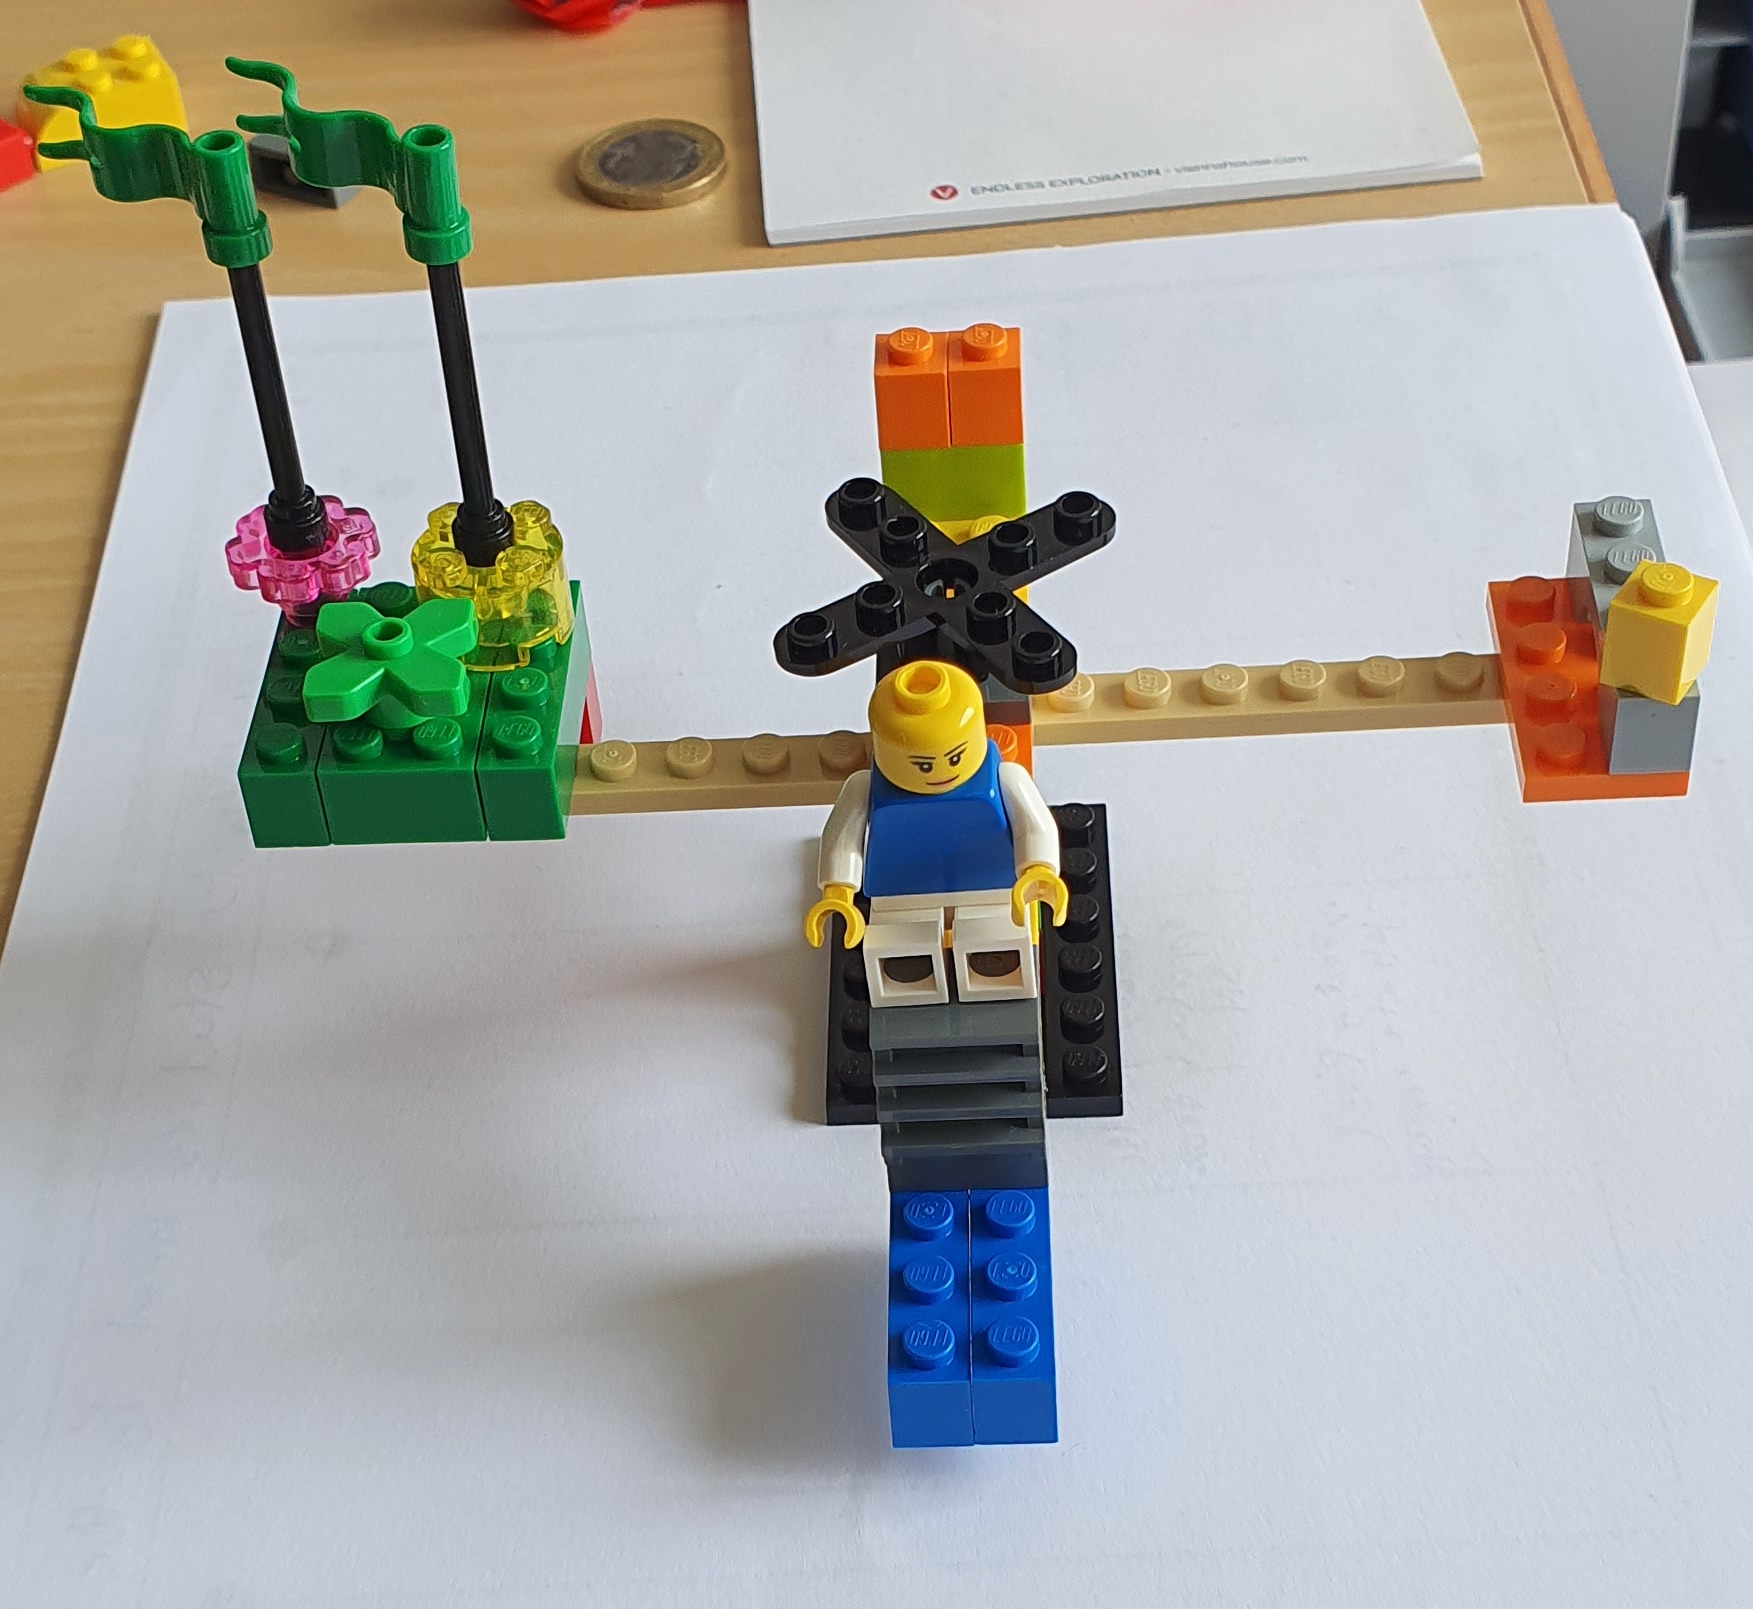
\includegraphics[width=7.7cm]{img/week_4.jpg}
        \end{center}
        \caption{``The game plan'' - Prototype of week 4}
        \label{fig:week4}
    \end{figure} 
\end{center}


\pagebreak

\end{document}